\documentclass{beamer}


\usepackage{color}
\usepackage{listings}
\usepackage{courier}
\lstset{
basicstyle=\tiny\ttfamily, % Standardschrift
numbers=left, % Ort der Zeilennummern
tabsize=4, % Groesse von Tabs
}
\lstloadlanguages{C++}
%\DeclareCaptionFont{blue}{\color{blue}}
 
%\captionsetup[lstlisting]{singlelinecheck=false, labelfont={blue}, textfont={blue}}
\usepackage{caption}
\DeclareCaptionFont{white}{\color{white}}
\DeclareCaptionFormat{listing}{\colorbox{8}{\parbox{\textwidth}{\hspace{15pt}#1#2#3}}}
\captionsetup[lstlisting]{format=listing,labelfont=white,textfont=white, singlelinecheck=false, margin=0pt, font={bf,footnotesize}}

\usepackage[utf8x]{inputenc}
\usepackage{ngerman}
\usepackage{graphicx}




\title{Diskrete Minimalflächen}
\author{Patrick Dabbert, Stephan Hilb und Martin Rösner}
\date{\today}

\usepackage{beamerthemesplit}


\begin{document}

\begin{frame}
	\titlepage
\end{frame}

\begin{frame}
	\frametitle{Inhaltsverzeichnis}
	\tableofcontents
\end{frame}

\section{Allgemeines}

\subsection{Die Aufgabe und unsere Interpretation}

\begin{frame}
	\frametitle{Die Aufgabenstellung}
	\begin{quote}
		„Beschreiben Sie eine triangulierte Fläche in eine gegeben gekrümmte Raumkurve ein und versuchen Sie, eine Approximation an eine Minimalfläche zu berechnen.“
	\end{quote}
\end{frame}

\begin{frame}
	\frametitle{Unsere Überlegungen dazu}
	\begin{itemize}
		\item
			Kurve in parametrisierter Form: $\gamma(t)$
		\item
			Zur Minimierung ist ein Dreiecksgitter nötig
			
			$\quad \implies$ Triangulierung erforderlich
		\item
			Einfaches Ausgabeformat für die Visualisierung
	\end{itemize}
\end{frame}

\subsection{Die Datenstrukturen}

\begin{frame}
	\frametitle{Vertex}
	\lstinputlisting{vertex.cpp}
\end{frame}

\begin{frame}
	\frametitle{Edge}
	\lstinputlisting{edge.cpp}
\end{frame}

\begin{frame}
	\frametitle{Triangle}
	\lstinputlisting{triangle.cpp}
\end{frame}

\subsection{Das Ausgabeformat für die Visualisierung}

\begin{frame}[fragile]
	\frametitle{Das Wavefront OBJ-Format}
	\begin{itemize}
		\item
			Spezifikation von Punkten im Raum durch Zeilen der Form
			\begin{verbatim}
v [x-Koordinate] [y-Koordinate] [z-Koordinate]
			\end{verbatim}
			Implizite Indizierung der Punkte nach ihrer Reihenfolge.
		\item
			Verbindungslinie durch $n$ Punkte:
			\begin{verbatim}
l [ID Punkt 1] [ID Punkt 2] ... [ID Punkt n]
			\end{verbatim}
		\item
			Dreiecksfläche, definiert durch drei Punkte:
			\begin{verbatim}
f [ID Punkt 1] [ID Punkt 2] [ID Punkt 3]
			\end{verbatim}
	\end{itemize}
\end{frame}

\begin{frame}[fragile]
	\frametitle{Beispiel}
	\begin{verbatim}
v 0 0 0
v 1 0 0
v 0 1 0
v 0 0 1
l 1 4
f 1 2 3
	\end{verbatim}
\end{frame}


\section{Triangulierung}

\begin{frame}
	\frametitle{Anfangsdreieck}

	Definiere ein Dreieck mit den Eckpunkten $\gamma(0), \gamma(\frac 13), \gamma(\frac 23)$.
	\begin{figure}
		\caption{Anfangstriangulierung bei einer Kreiskurve}
		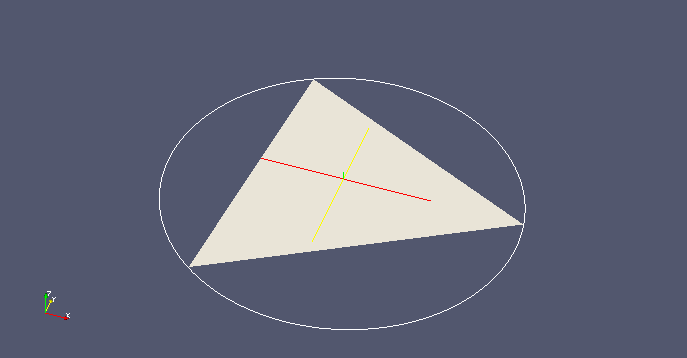
\includegraphics[width=0.8 \linewidth]{kreis0.png}
	\end{figure}
\end{frame}

\begin{frame}
	\frametitle{Vorgehen}

	\begin{enumerate}[1.]
		\item
			Halbiere jede Seite (erzeuge neuen Punkt auf der Mitte)
		\item
			Falls die Seite eine Randseite war, verschiebe den Mittelpunkt auf die Randkurve
		\item
			Erzeuge neue Dreiecke durch die eben definierten Punkte.
	\end{enumerate}
\end{frame}

\begin{frame}
	\frametitle{Kreiskurve}

	\begin{figure}
		\caption{Kreistriangulierung nach erstem Vierteln}
		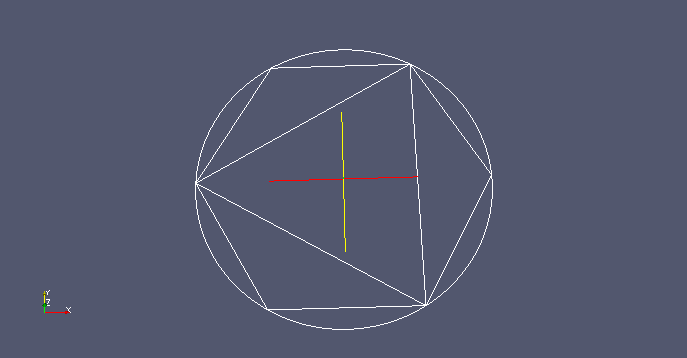
\includegraphics[width=0.8 \linewidth]{kreis1.png}
	\end{figure}
\end{frame}

\begin{frame}
	\frametitle{Kreiskurve}

	\begin{figure}
		\caption{Kreistriangulierung nach zweitem Vierteln}
		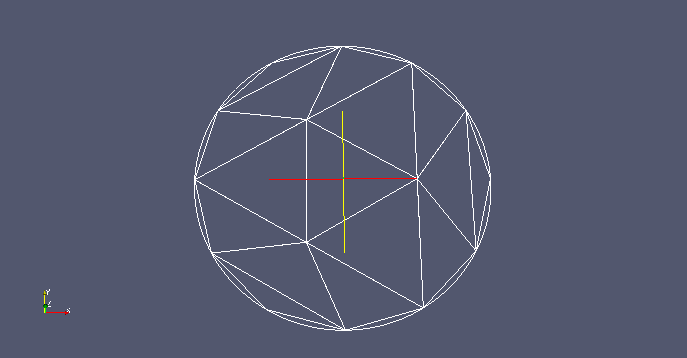
\includegraphics[width=0.8 \linewidth]{kreis2.png}
	\end{figure}
\end{frame}


\section{Minimierung}

\begin{frame}
	\begin{itemize}
		\item
			Betrachte nach jedem Verfeinerungsschritt nacheinander alle freien (nicht auf dem Rand liegende) Knoten
		\item
			Für jeden Knoten: verschiebe so, dass die Fläche aller angrenzenden Dreiecke minimial wird
		\item
			Wiederhole das, solange die Gesamtfläche bei jedem Schritt um einen gewissen Prozentsatz minimiert wird.
	\end{itemize}
\end{frame}

\begin{frame}
	\frametitle{Pseudecode Beispiel}
	\lstinputlisting{minalg.cpp}
\end{frame}

\subsection{Das lokale Minimierungsproblem}

\begin{frame}
	\begin{itemize}
		\item
			Was ist die optimale oder eine gute Verschiebung?
		\item
			Welche Implementierungsmöglichkeiten gibt es?
	\end{itemize}
\end{frame}

\begin{frame}
	\frametitle{Mögliche Ansätze}
	\begin{itemize}
		\item
			Koordinaten der umliegenden Dreieckseckpunkte in irgendeiner Weise „mitteln“
		\item
			Das mathematische Minimierungsproblem lösen
		\item
			Ein Näherungsverfahren verwenden (z.B. ein Gradientenverfahren)
	\end{itemize}
\end{frame}

\subsection{Das Gradientenverfahren}

\begin{frame}
	\frametitle{Der Algorithmus}
	\begin{enumerate}[1.]
		\item
			Berechne den Gradienten des Flächeninhalts der umliegenden Dreiecke in Abhängigkeit des aktuellen Punktes
		\item
			Prüfe, ob die Fläche sich verkleinert, wenn der Punkt um den Gradient verschoben wird.
			Wenn ja: Verschiebe den Punkt.
			Wenn nein: Halbiere den Gradienten.
		\item
			Wiederhole 2. so lange, bis eine Verschiebung stattfindet
	\end{enumerate}
\end{frame}

\begin{frame}
	\frametitle{Code Beispiel}
	\lstinputlisting{mingradient.cpp}
\end{frame}

\begin{frame}
	\frametitle{Berechnung des Gradienten für ein Dreieck}
	Minimiere das Dreieck $x_0,x_1,x_2$, verschiebe dabei $x_0$.

	Der Gradient ist durch die Höhe des Dreiecks durch $x_0$ in Richtung der gegenüberliegenden Grundseite gegeben.
	Konkret:
	\[
		\big((x_0 - x_1) \times (x_0 - x_1)\big) \times (x_1 - x_2);
	\]
\end{frame}

\begin{frame}
	\frametitle{Code}
	\lstinputlisting{grad.cpp}
\end{frame}


\section{Ergebnisse}

\begin{frame}
	\frametitle{Schöne Fläche}
	Die meisten geschlossenen Kurven, ohne Überschneidungen liefern gute Ergebnisse.
\end{frame}

\begin{frame}
	\frametitle{Weniger schöne Flächen}
	Probleme bereiten
	\begin{itemize}
		\item
			offene Kurven 
		\item
			Kurven mit Überschneidungen (Viviani)
		\item
			Fälle, in denen die Triangulierung zu stark verzerrt wird
	\end{itemize}
\end{frame}

\begin{frame}
	\frametitle{Weiterführende Überlegungen}	
	\begin{itemize}
		\item
			Verbesserung der Struktur des Dreiecksnetzes (möglichst gleichseitige Dreiecke)
		\item
			Bisektion statt Viertelung zur Netzverfeinerung
		\item
			Andere Strategien für die Punktverschiebung
	\end{itemize}
\end{frame}

\begin{frame}[fragile]
	\frametitle{Ende}
	Der Quellcode und diese Prästentation sind zu finden auf
	\begin{verbatim}
		https://github.com/stev47/cp/tree/master/projekt1
	\end{verbatim}
\end{frame}




\end{document}
